%%%%%%%%%%%%%%%%%%%%%%%%%%%%%%%%%%%%%%%%%%%%%%%%%%%%%%%%%%%%%%%%%%%%%%
%     File: ExtendedAbstract_backg.tex                               %
%     Tex Master: ExtendedAbstract.tex                               %
%                                                                    %
%     Author: Andre Calado Marta                                     %
%     Last modified : 27 Dez 2011                                    %
%%%%%%%%%%%%%%%%%%%%%%%%%%%%%%%%%%%%%%%%%%%%%%%%%%%%%%%%%%%%%%%%%%%%%%
% A Theory section should extend, not repeat, the background to the
% article already dealt with in the Introduction and lay the
% foundation for further work.
%%%%%%%%%%%%%%%%%%%%%%%%%%%%%%%%%%%%%%%%%%%%%%%%%%%%%%%%%%%%%%%%%%%%%%

\section{Background}
\label{sec:backg}
We begin by providing some of the financial background required to understand the later results.

\subsection{Option payoffs and prices}
From the definition of a European option we can deduce the payoff function of this contract as
\begin{subequations}\label{callput}
\begin{align}
&\text{Payoff}_{Euro,\ call}(K,T)=\max\left(S(T)-K,0\right);\\
&\text{Payoff}_{Euro,\ put}(K,T)=\max\left(K-S(T),0\right),
\end{align}
\end{subequations}
\noindent where $K$ is the option's strike price and $S(T)$ is the asset's price, $S(t)$, at the maturity, $T$.


An up-and-in Barrier option's payoff function is exactly as shown in eq.\eqref{callput} conditioned on a given threshold $B$ being surpassed at any point until the maturity (i.e. $\exists\,t<T\,:\,S(t)>B$). It should be zero otherwise.
The influence of this threshold $B$ on the option price is trivial: because it is linked to the probability of the stock price reaching $B$, the higher the barrier $B$, the lower the corresponding option price.

We can price options by setting their expected profit to be the same as a risk-neutral investment, (e.g. bank deposit). The price of an option can thus be deduced as it's expected future payoff, discounted back to the present
\begin{equation}\label{pricepayoff}
\text{Price}(K,T)=e^{-rT}\mathbb{E}\left[\text{Payoff}(K,T)\right],
\end{equation}
\noindent where $r$ is the risk-free interest rate, defined as the interest an investor would receive from any risk-free investment (e.g. treasury bills). In general, this rate changes slightly with time and is unknown.

\subsection{Black-Scholes Formulae}
Fischer Black and Myron Scholes developed a mathematical model to price European options - the famous Black-Scholes (BS) model~\citep{Scholes} - still in use in present days~\citep{Wilmott3}.

This model states that the price of a European option follows the partial differential equation
\begin{equation}\label{BS2}
\pdv{V}{t}+\frac{1}{2}\sigma^2S^2\pdv{^2V}{S^2}+rS\pdv{V}{S}-rV=0,
\end{equation}
\noindent where $V$ is the price of the option and $\sigma$ is the stock price volatility, which affects how erratically the stock price moves. The interest rate, $r$, is assumed to be a known function of time, and the volatility, $\sigma$, is assumed to be a known constant.

Under this model, we assume that stock prices follow a Geometric Brownian Motion (GBM), defined as
\begin{equation}\label{GBM}
dS(t)=rS(t)dt+\sigma S(t)dW(t),
\end{equation}
\noindent with $\{W(t),\ t>0\}$ defining a one-dimensional Brownian motion. An example of such processes is represented in \autoref{fig:GBM}.

\begin{figure}[H]
    \centering
      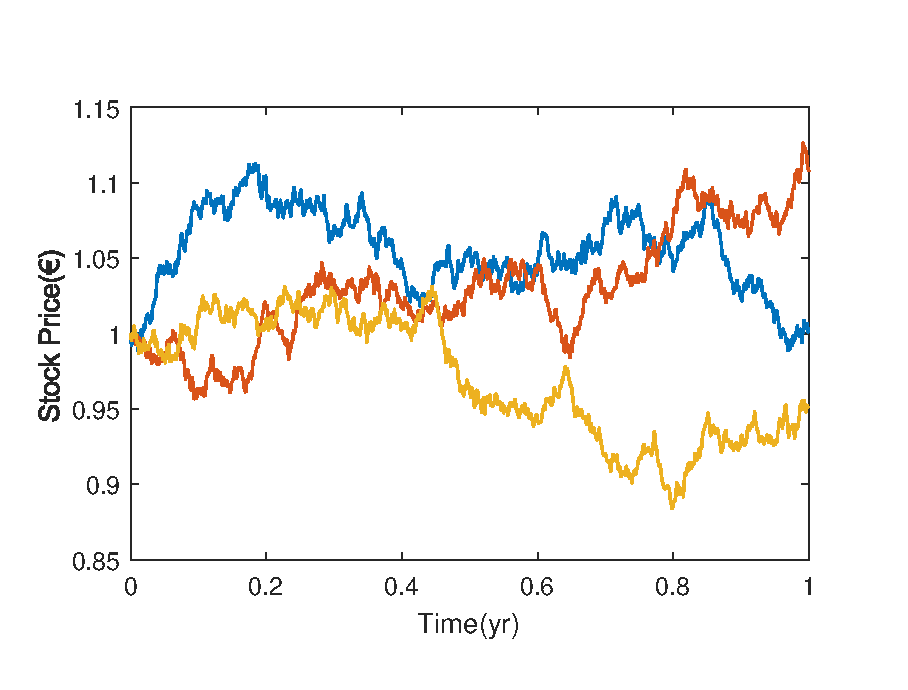
\includegraphics[width=.8\columnwidth,trim={0.35cm 0.6cm 1.4cm 1.35cm},clip]{GBM.eps}
      \caption{Example of three realizations of a Geometric Brownian Motion process.}\label{fig:GBM}
    \end{figure}
    
To price options, we need to solve the PDE in eq.\eqref{BS2} as we would for the diffusion equation's initial value problem~\citep{Dilao}, resulting in
\begin{subequations}\label{callputBS}
\begin{align}
&C(K,T)=N(d_1)S_0-N(d_2)Ke^{-rT};\\
&P(K,T)=-N(-d_1)S_0+N(-d_2)Ke^{-rT},
\end{align}
\end{subequations}
\noindent where $N(\cdot)$ is the cumulative distribution function of the standard normal distribution and where $d_1$, $d_2$ are given by
\begin{subequations}\label{d1d2}
\begin{align}
&d_1=\frac{1}{\sigma\sqrt{T}}\left[\log\left(\frac{S_0}{K}\right)+\left(r+\frac{\sigma^2}{2}\right)T\right];\\
&d_2=d_1-\sigma\sqrt{T}.
\end{align}
\end{subequations}


In \autoref{fig:Inception} we represent the prices of call and put options at both the inception (i.e. $t=0$) and maturity as a function of the ratio $K/S_0$.
\begin{figure}[H]
    \centering
      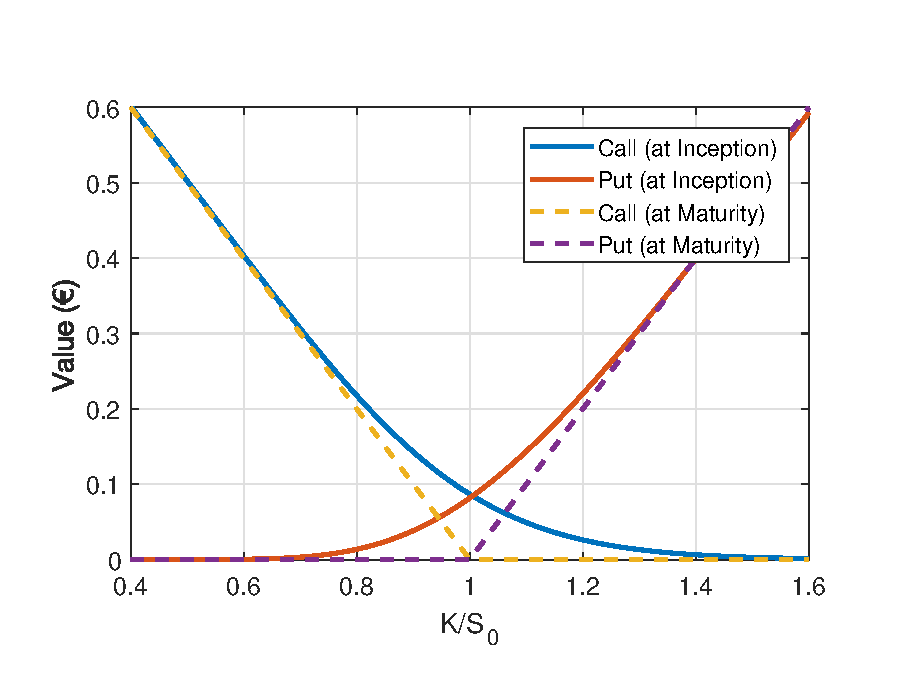
\includegraphics[width=.8\columnwidth,trim={0.6cm 0.4cm 1.15cm 1.4cm},clip]{Inception.eps}
      \caption{Call and Put option values at inception and maturity}\label{fig:Inception}
    \end{figure}

We can thus use eqs.\eqref{callputBS} to precisely price European options, so long as all the parameters are exactly known and remain constant throughout the option's duration (which is never true).